%Gesammtübersicht Fragestellung
Während der Messwoche der geophysikalischen Geländeübungen wurden vier verschiedenen Messmethoden verwendet: die Refraktionsseismik, Geoelektrik, Gravimetrie und Magnetik. An erster Stelle stand bei
uns die Fragestellung, inwieweit sich die Ergebnisse dieser Messmethoden unterscheiden. Dadurch wollten wir die Messverfahren besser verstehen und einschätzen können, welchen Einfluss die Wahl des Messverfahrens auf die Ergebnisse hat. Bei jedem Profil wurden der Anfangs- und Endpunkt markiert und dann am letzten Tag während der Gravimetrie-Messung mit einem GPS-Gerät vermessen. Die Koordinaten all dieser Punkte sind im Anhang in Tabelle \ref{tab:gps1} aufgelistet.

Wie bereits in Kapitel \ref{sec:Messgebiete} \nameref{sec:Messgebiete} beschrieben, wird unter Messgebiet 1 ein Basaltgang vermutet. Unser zweites Ziel war es, dessen Lage möglichst genau zu bestimmen. 

Wir wussten zwar, dass der Basaltgang eigentlich nicht mit der Seismik vermessen werden kann,
wollten dies aber überprüfen und herausfinden, inwiefern unsere Messergebnisse durch den Basaltgang beeinflusst worden sein könnten. Das Profil, auf dem die Messung durchgeführt wurde, ist in 
Abbildung \ref{abb:Seismik} als S21-S22 zu sehen.
Die Seismik-Messung auf Messgebiet 2 wurde durchgeführt, um ein Verfahren zu haben, mit dem die Geoelektrik-Messung verglichen werden kann und um gute Ergebnisse für die Auswertung zu haben.
Das Profil S31-S32 auf Messgebiet 2 war relativ lang und eben, wie man in Abbildung \ref{abb:Seismik} erkennt, sodass wir davon ausgingen, hier gut eine Schichtgrenze finden zu können.

\begin{figure}[ht]
 \centering
 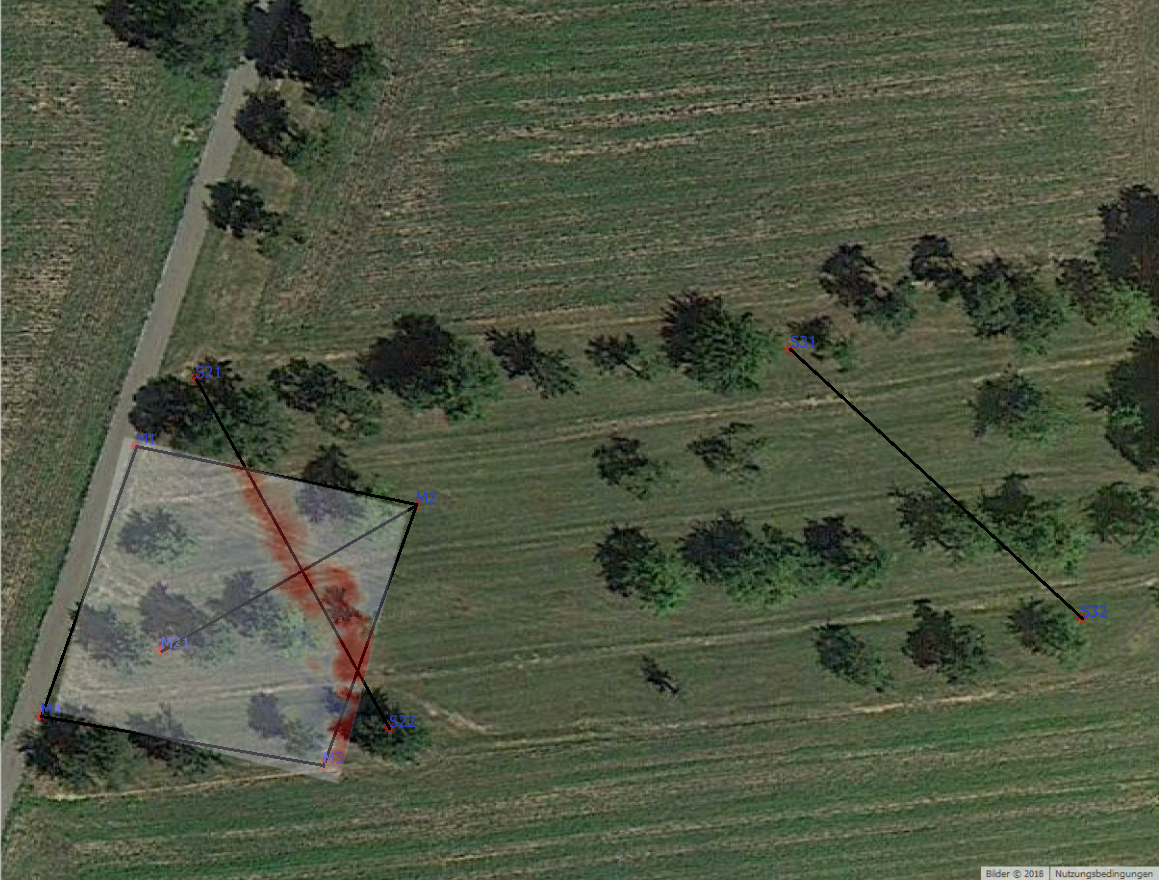
\includegraphics[width=0.9\textwidth]{fig/Seismik.png}
 \caption[Seismik- Messprofile S11-S21 und S21-S22]{Seismik-Messprofile S11-S21 und S21-S22. Die Graphik wurde von Katharina Adrion und Niels Gieseler übernommen.}
 \label{abb:Seismik}
\end{figure}

Die Magnetik wurde am ersten Tag durchgeführt. Hier war es uns bei der Kartierung wichtig, zunächst die Lage des Basaltgangs festzustellen, um darauf aufbauend alle weiteren Messungen durchführen zu können.
Das Gebiet, auf dem die Kartierung zu sehen ist, ist in Abbildung \ref{abb:Kart} abgebildet. Die restlichen Messungen wurden auf den Profilen, die in Abbildung \ref{abb:Magnetik} eingezeichnet durchgeführt.
Hier war unsere Fragestellung wieder, wie gut sich die Magnetik im Vergleich zu den anderen Messverfahren zum Lokalisieren des Basaltgangs eignet.

\begin{figure}[ht]
 \centering
 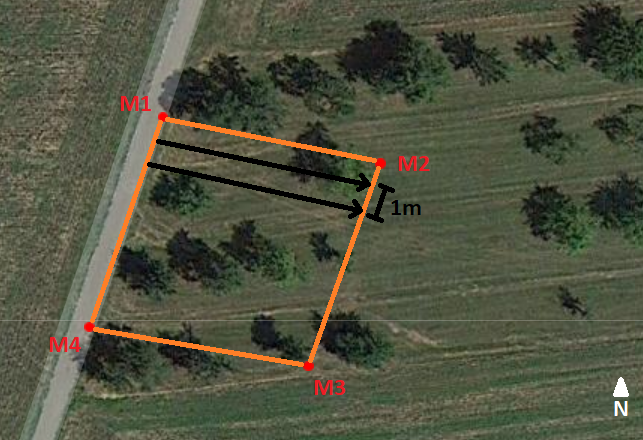
\includegraphics[width=0.9\textwidth]{fig/Kartierunggps.png}
 \caption[Lage der Magnetik-Kartierung]{Lage der Magnetik-Kartierung. Die Graphik wurde von Rebekka Kirchgässner und Luisa Rank übernommen.}
 \label{abb:Kart}
\end{figure}

\begin{figure}[ht]
 \centering
 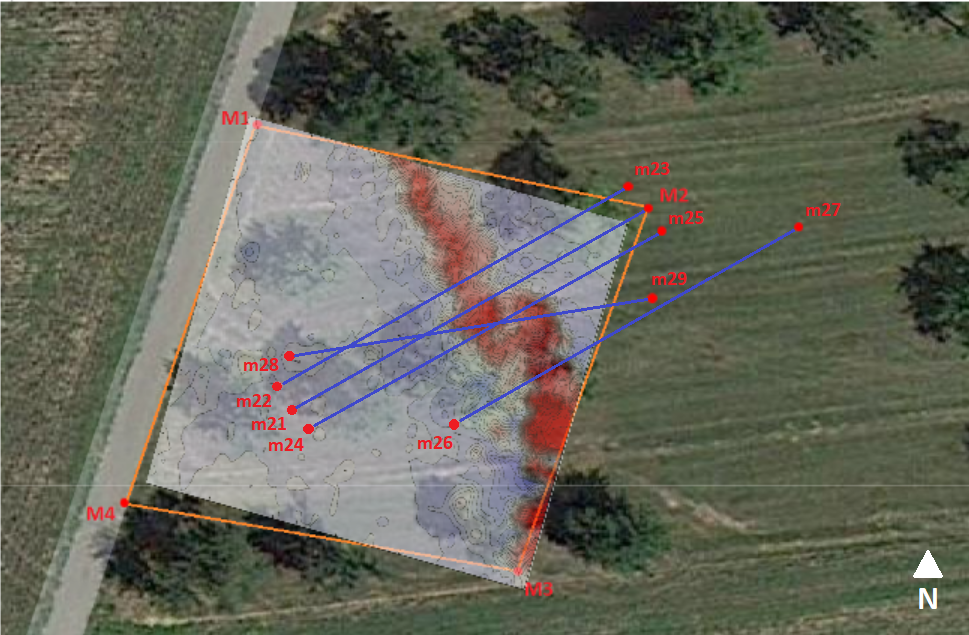
\includegraphics[width=0.9\textwidth]{fig/MagnetikGesamtueberblick.png}
 \caption[Gesamtübersicht über die Profile der Magnetik]{Gesamtübersicht über die Profile der Magnetik. Die Graphik wurde von Rebekka Kirchgässner und Luisa Rank übernommen.}
 \label{abb:Magnetik}
\end{figure}

Bei der Geoelektrik wurden wieder auf beiden Messgebieten Messungen durchgeführt. Die Sondierung wurde entlang des Seismik-Profils in Messgebiet 2 durchgeführt. Dies ist in 
Abbildung ??? eingezeichnet. Die Messung wurde durchgeführt, um zu sehen, ob wir Schichtgrenzen finden und wenn ja, ob diese mit denen der Seismik übereinstimmen.
Die Tomographie und Wenner-Kartierung (Profil E11-E12) wurden, wie schon die Messungen der Magnetik und Gravimetrie, orthogonal zum Basaltgang durchgeführt, um die Messergebnisse dieser drei Verfahren
miteinander vergleichen zu können. Die beiden Profile sind in Abbildung \ref{abb:Geoelek} abgebildet.

\begin{figure}[ht]
 \centering
 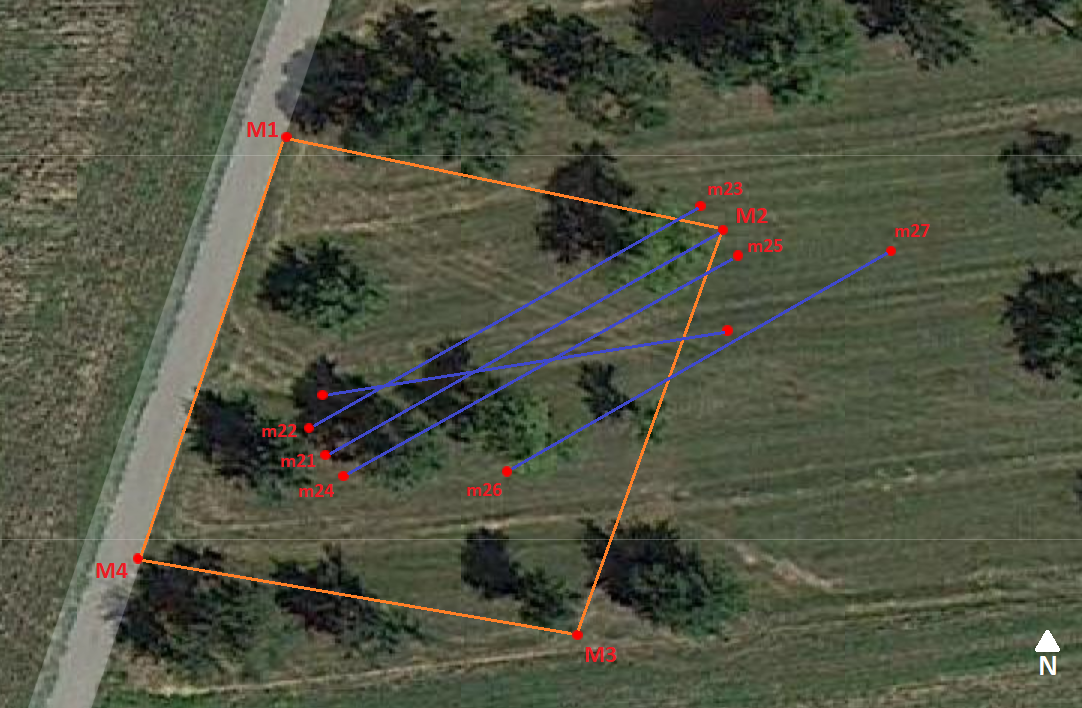
\includegraphics[width=0.9\textwidth]{fig/Profilegps.png}
 \caption[Profil E21-E22 der Geoelektrik und Profil S11-S12 der Seismik]{Profil E21-E22 der Geoelektrik und Profil S11-S12 der Seismik. Die Graphik wurde von Rebekka Kirchgässner und Luisa Rank übernommen.}
 \label{abb:Geoelek}
\end{figure}

\begin{figure}[ht]
 \centering
 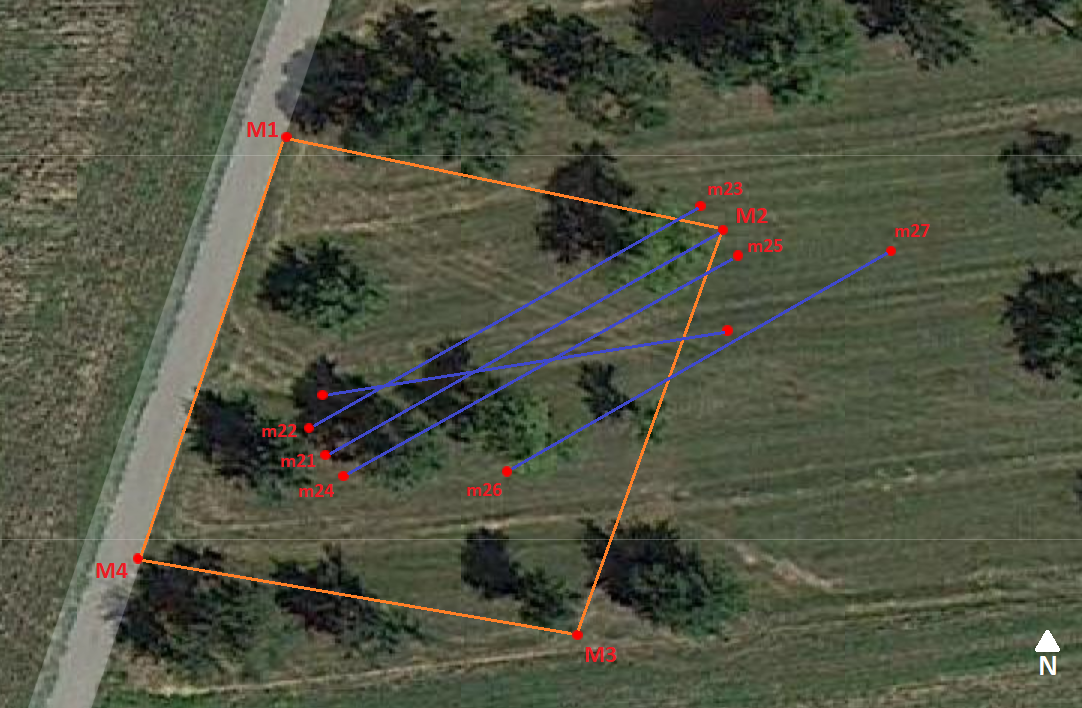
\includegraphics[width=0.9\textwidth]{fig/Profilegps.png}
 \caption[Profile der Geoelektrik]{Profile der Geoelektrik. Die Graphik wurde von Rebekka Kirchgässner und Luisa Rank übernommen.}
 \label{abb:Geoelek}
\end{figure}

Da die Gravimetrie-Messung sehr viel Zeit gebraucht hat, wurde nur eine Messung auf Profil G0-G16, zu sehen in Abbildung \ref{abb:Geoelek2}, durchgeführt. Wir erhofften uns, genau genug
messen zu können, um den Basaltgang zu sehen und eventuell ähnliche Ergebnisse wie die bereits beschriebenen Messmethoden zu haben.

\begin{figure}[ht]
 \centering
 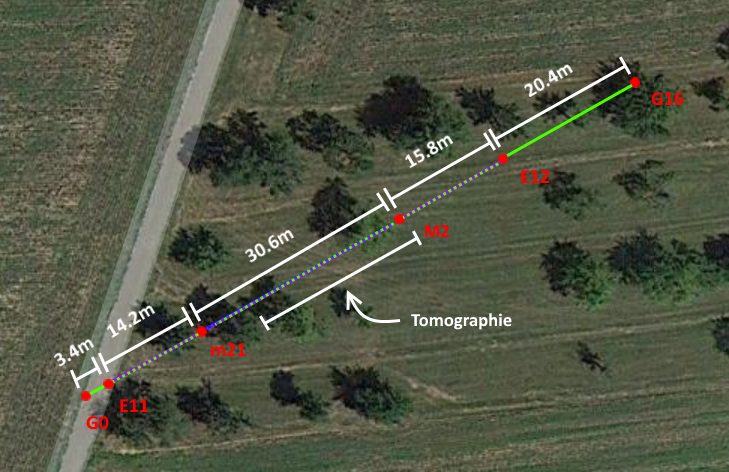
\includegraphics[width=0.9\textwidth]{fig/ElektrikMagnetikGravimetrie.png}
 \caption[Profil der Gravimetrie]{Profil der Gravimetrie. Die Graphik wurde von Rebekka Kirchgässner und Luisa Rank übernommen.}
 \label{abb:Geoelek2}
\end{figure}